\documentclass{boi2014-dk}

\usepackage{enumitem}

\renewcommand{\DayNum}{2}
\renewcommand{\TaskCode}{postmen}
\renewcommand{\TaskName}{Senior Postmen}
\renewcommand{\TaskVersion}{0.1}

\begin{document}
    \begin{wrapfigure}[8]{r}{4cm}
        \vspace{-18pt}
		\includegraphics[width=4cm]{\TaskCode.jpeg}
	\end{wrapfigure}

    Det er år 2036 og europa er fyldt af pensionister. For at holde dem sunde
    har det europæiske ministerium for flertal (pensionister \emph{er} et
    flertal!) foreslået at få dem til at aflevere den lille mængde brevpost
    der stadig sendes -- typisk til pensionister. Dette foreslag vil blive
    implementeret i hele Europa, selv i de frie stater Norge og Schweiz.

    Ministeriet har udtænkt et "pensionist postbud system" på følgende måde:
    Europa er indelt i postdistrikter. Et postdistrikt har et vejnetværk af
    gader og vejkryds. Man kan gå begge veje af hver gade i netværket. I hvert
    distrikt er der vilkårligt mange pensionister, der kan hyres som postbud.
    Hver morgen modtager hvert postbud en taske med post, der skal leveres på
    en tur, der dækker en del af vejnetværket. Hver tur skal være
    pensionistvenlig, dvs. den skal opfylde følgende betingelser:

    \begin{itemize}
        \item Den starter og slutter ved samme vejkryds. (Hey, det er en
            tur!)
        \item Den går aldrig igennem samme vejkryds to gange. (Pensionisterne
            må ikke blive forvirrede).
        \item Den må ikke have en gade til fælles med nogen anden tur. Så hver
            gade i distriktet bliver besøgt af netop et postbud.
    \end{itemize}

    Tilsammen skal turene dække det givne vejnetværk: Hver gade i
    vejnetværket skal være del af netop en tur.

    \Task
    Ministeriet har nu brug for software, der for et givet postdistrikts
    vejnetværk, viludregne en mængde af pensionistvenlige ture, der
    dække netværket.

    \Input
    Inputtet beskriver vejnetværket.

    Den første linje indeholder to heltal $N$ og $M$. $N$ er antallet af
    vejkryds og $M$ er antallet af gader. Vejkrydsene er nummereret fra
    $1$ til $N$.

    Hver af de følgende $M$ linjer indeholder to heltal $U$ og $V$, der
    betyder at der er en gade der forbinder vejkryds $U$ og $V$.

    For ethver input holder det at:

    \begin{enumerate}
        \item For alle par af vejkryds kan du gå fra det ene vejkryds til
            det andet.
        \item Der findes en løsning. Dvs.~der findes en mængde af
            pensionistvenlige ture, der dækker vejnetværket.
    \end{enumerate}

    \Output
    Den første linje af outputtet skal indeholde et heltal $T$, antallet
    af ture.

    De $T$ ture skal beskrives på de følgende $T$ linjer.
    Hver af disse linjer skal starte med et heltal $C$, der beskriver antallet
    af forskellige vejkryds postbuddet skal passere på turen.
    De følgende $C$ heltal på linjen er numrene på vejkrydsene på turen.
    De skal skrives i den rækkefølge som vejkrydsene bliver besøgt af
    postbuddet, sådan at det startende (og sluttende) vejkryds bliver
    skrevet først (og kun en gang).

    Hvis der er to eller flere løsninger, må dit program udskrive en vilkårlig
    en af dem.

    \Example

    \example
    {
        10 15 \newline
        1 2 \newline
        5 1\newline
        2 3 \newline
        9 2\newline
        3 4 \newline
        6 3\newline
        4 5 \newline
        7 4\newline
        4 8 \newline
        5 7 \newline
        8 5\newline
        6 7 \newline
        7 8 \newline
        8 10 \newline
        10 9
    }
    {
        3 \newline
        7 2 3 4 5 8 10 9 \newline
        3 4 7 8 \newline
        5 1 5 7 6 3
    }
    {
        Det følgende billede illustrerer vejnetværket og de tre
        pensionistvenlige ture, som kan bruges til at dække det.

        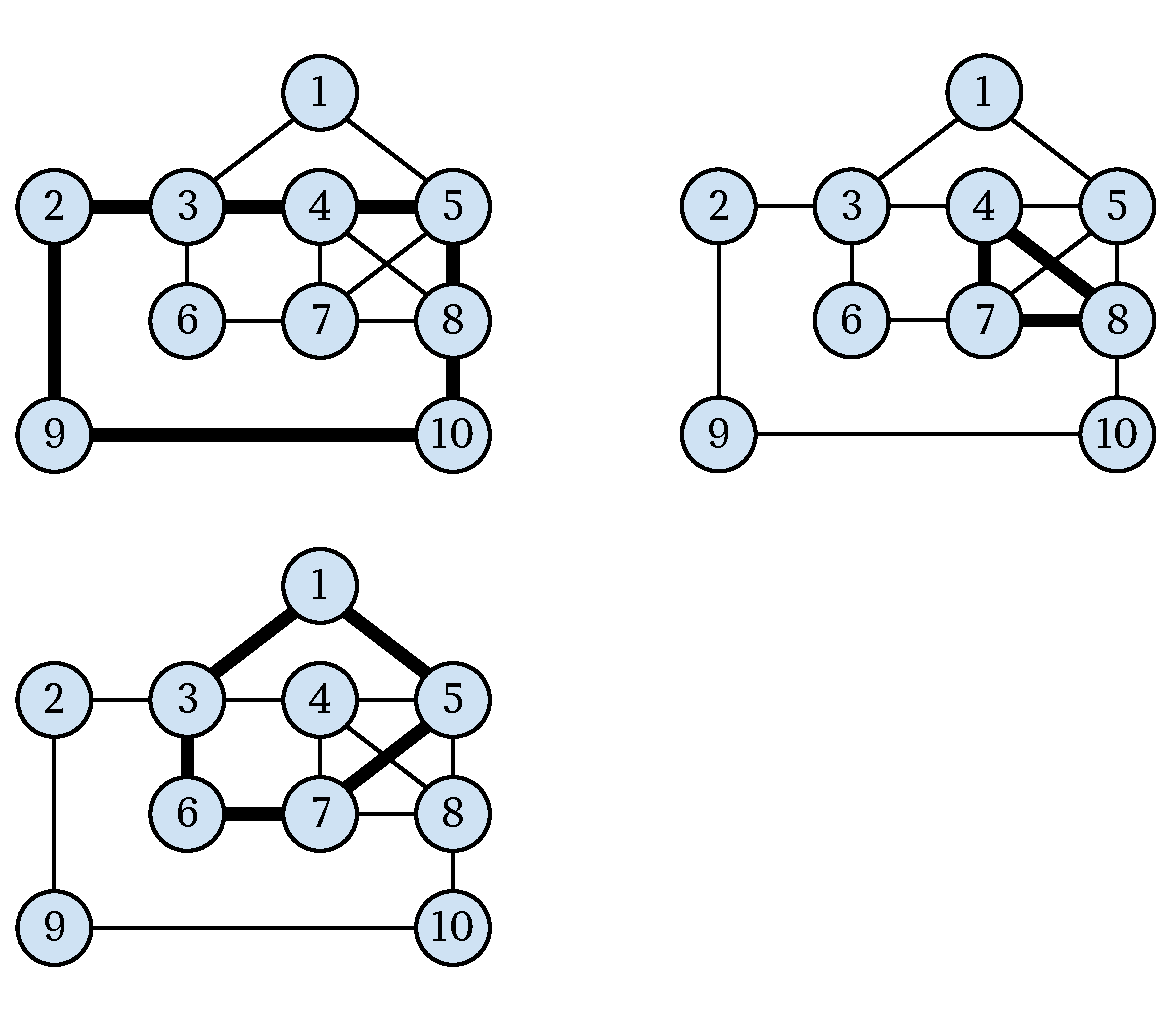
\includegraphics[width=7cm]{senior-example}

        Bemærk at der er flere løsninger til dette eksempel, hvoriblandt
        en af dem kun indeholder to ture.
    }

    \Scoring

    \begin{description}
        \item[Delopgave 1 (40 point):] $1 \le N \le 2\ 000$, $1 \le M \le 100\ 000$.
        \item[Delopgave 2 (20 point):] $1 \le N \le 100\ 000$, $1 \le M \le 100\ 000$.
        \item[Delopgave 3 (40 point):] $1 \le N \le 500\ 000$, $1 \le M \le 500\ 000$.
    \end{description}

    \Constraints

    \begin{description}
        \item[Tidsbegrænsning:] 1 s.
        \item[Hukommelsesbegrænsning:] 256 MB.
    \end{description}

\end{document}
